\documentclass[a4paper]{report}

\usepackage[latin1]{inputenc}
\usepackage[T1]{fontenc}
\usepackage[francais]{babel}
\usepackage{setspace}
\usepackage{url}
\usepackage{amsmath}
\usepackage{amssymb}
\usepackage{mathrsfs}
\usepackage{graphicx}

\title{Homework 4 and Queing Lab}
\author{Achille \textsc{Sala\"{u}n}}

\begin{document}

\maketitle
\section*{Problem 1}
\subsection*{Question 1}
Let set $\lambda=\lambda_{n}+\lambda_{f}$, $\mathbb{E}[S_{n}]=\frac{10 Mbit}{10 Mbps}=1s$ and $\mathbb{E}[S_{f}]=\frac{5 Mbit}{1 Mbps}=5s$. \\

So, the mean transmission time overall $\mathbb{E}[S]$ is equal to :
\[\mathbb{E}[S] = \frac{\lambda_{n}}{\lambda} \mathbb{E}[S_{n}]+\frac{\lambda_{f}}{\lambda} \mathbb{E}[S_{f}] = 2,14s\]

Thus, by definition, the utilization $\rho$ of this system is equal to :
\[\rho = \lambda \mathbb{E}[S] = 0,75\]

%---------------------------------------------------------------------------
\subsection*{Question 2}
Because of the FCFS scheduling, the mean queuing time for requests doesn't depend on its origin (if the request is a far or near user request). Let derive it first : 
\[\mathbb{E}[T_{Q}]=\rho \mathbb{E}[S_{E}]+\mathbb{E}[N_{Q}] \mathbb{E}[S] = \frac{\rho}{1-\rho}\mathbb{E}[S_{E}]\]
We have :
\[\mathbb{E}[S_{n}^{2}]=(1+c_{v,n}^{2})\mathbb{E}[S_{n}]^{2} = 5s^{2}\] 
\[\mathbb{E}[S_{f}^{2}]=(1+c_{v,f}^{2})\mathbb{E}[S_{f}]^{2} = 50s^{2}\]
So : 
\[\mathbb{E}[S^{2}]= \frac{\lambda_{n}}{\lambda} \mathbb{E}[S_{n}^{2}]+\frac{\lambda_{f}}{\lambda} \mathbb{E}[S_{f}^{2}] = 17,857s^{2}\]
We can now compute :
\[\mathbb{E}[S_{E}]=\frac{\mathbb{E}[S^{2}]}{2 \mathbb{E}[S]}=4,167s\] 
Finally, the mean queuing time for requests is :
\[\mathbb{E}[T_{Q}]=12,5s\]

In conclusion, the mean download time of files to near users is $\mathbb{E}[T_n]=\mathbb{E}[T_{Q}]+\mathbb{E}[S_{n}]=13,5s$ and the mean download time of files to far users is $\mathbb{E}[T_f]=\mathbb{E}[T_{q}]+\mathbb{E}[S_{f}]=17,5s$.

%---------------------------------------------------------------------------
\subsection*{Question 3}
And so the mean download time overall is $\mathbb{E}[T]=\mathbb{E}[T_{Q}]+\mathbb{E}[S]=14,64s$.

%---------------------------------------------------------------------------
\subsection*{Question 4}
In the case of the same queue implementing the Processor-Sharing scheduling rather the First Come First Served one, the mean download time overall would be : 

\[\mathbb{E}[T] = \frac{\mathbb{E}[S]}{1- \rho} = 8,56s \]
%***************************************************************************
\newpage
\section*{Problem 2}
From the course, we get : \\
\begin{description}
\item[$(01)\leftrightarrow (e)$ :] $\mathbb{E}[T]^{M/G/1/FCFS} = \frac{\rho}{1-\rho} \mathbb{E}[S_{E}]+\mathbb{E}_{S}$
\item[$(02)\leftrightarrow (c)$ :] $\mathbb{E}[T]^{M/G/1/PS} = \frac{\mathbb{E}[S]}{1-\rho} $
\item[$(03)\leftrightarrow (e)$ :] $\mathbb{E}[T]^{M/G/1/LCFS} =\frac{\rho}{1-\rho} \mathbb{E}[S_{E}]+\mathbb{E}_{S}$
\item[$(04)\leftrightarrow (c)$ :] $\mathbb{E}[T]^{M/G/1/PLCFS} =\frac{\mathbb{E}[S]}{1-\rho}$
\item[$(05)\leftrightarrow (e)$ :] $\mathbb{E}[T]^{M/M/1/FCFS} =\frac{\rho}{1-\rho} \mathbb{E}[S_{E}]+\mathbb{E}_{S}$
\item[$(06)\leftrightarrow (c)$ :] $\mathbb{E}[T]^{M/M/1/PS} =\frac{\mathbb{E}[S]}{1-\rho}$
\item[$(07)\leftrightarrow (g)$ :] \textit{None of the above}
\item[$(08)\leftrightarrow (a)$ :] $\rho = \lambda \mathbb{E}[S]$
\item[$(09)\leftrightarrow (c)$ :] $\mathbb{E}[B]^{M/G/1/FCFS} =\frac{\mathbb{E}[S]}{1-\rho}$
\item[$(10)\leftrightarrow (c)$ :] $\mathbb{E}[B]^{M/M/1/FCFS} =\frac{\mathbb{E}[S]}{1-\rho}$
\item[$(11)\leftrightarrow (b)$ :] $\mathbb{E}[S_{E}] = \frac{\mathbb{E}[S^{2}]}{2 \mathbb{E}[S]}$
\item[$(12)\leftrightarrow (b)$ :] $\mathbb{E}[W]^{M/G/1/FCFS} = \frac{\mathbb{E}[S^{2}]}{2 \mathbb{E}[S]}$

\end{description}
%***************************************************************************
\newpage
\section*{Queuing Lab}
\subsection*{Overview}
I did this lab thanks to a project, coded in Java, three teammates and I have realized. The goal of this project was to implement from scratch a simulator of discrete events with a scheduler. Our main concern in this project was to be as general as possible : \textbf{you should be able to design any network of M/M/1/FCFS, M/G/1/FCFS and M/G/1/SJF you want to.} However, since I focused on answering to the lab's questions, I didn't take care of, for example, how an item chooses an exit rather than an other one : it may be some mistakes despite the code run for networks more complicated than the system [Source $\rightarrow$ Queue $\rightarrow$ Pit].
\par
I have reorganized the lab in 4 packages : 
\begin{description}
\item[\texttt{theory} :] There is the class \texttt{Theory} which contains static methods returning the theoretical expected time spent in the queue (queuing and being served), for M/M/1, M/G/1/FCFS and M/G/1/SJF queues.

\item[\texttt{scheduler} :] Here are all the classes linked to the scheduler. They allow to build networks and then make the scheduler run by using the notion of events. Using this package leads to really verbose results, explaining what happens in each event.

\item[\texttt{schedulerNoText} :] This package is a copy of the previous one. However, all the \texttt{System.out.println("...");} has been removed in order to soar the run speed of the scheduler.

\item[\texttt{mains} :] Here are the three main classes I ran. Two are really interesting : \texttt{Main} which gives a verbose history while running the scheduler for a given $\rho$, and \texttt{MainNoText} which has been used for getting the results presented a bit later in this report.
\end{description}
\subsubsection{Scheduler}
A scheduler is a list of events. An event is an object containing the following pieces of information : who ? what ? when ? from where ? to where ? Recursively, the scheduler will execute the method \texttt{nextEvent()}, that is to say : looking for the next event, calling the actor supposed to execute the event, asking to this actor to do what he has to do.

\subsubsection{Actor}
Since the actor has been asked to execute the task he has to do with \texttt{execute()}, he will first look for which kind of action he's supposed to do. \\ 
\par
The systems we can study are items moving inside networks of cases (boxes). Both cases and items are actors.

\subsubsection{Cases}
They are the canvas of the system. Cases design a network, pointing on other cases. Thus, the list of cases pointing on me are my entrances and the list of cases I'm pointing on are my exits. A case A is pointing to a case B thanks to the command : \texttt{A.linkExit(B) ;} 
Cases contains Items which moves from case to case. There are basically three main kinds of cases : sources, queues and pits :

\begin{description}
\item[\texttt{Source} :] Typically, sources create new items. Actually there is two actions that a source can execute : \texttt{generate()} and \texttt{stop()}. The method \texttt{generate()} creates a new item, stores it in the case and plans the date when the item will go from the case following an exponential law. As soon as the item leave, a new generation begins. Thus, since the time between departures from the source is exponential : the law of arrival in the system is a Poisson law. \texttt{stop()} ends the simulation emptying the scheduler. If the sources are the only one to be able to do such an action, it's only because they are the only one to be absolutely necessary to run a simulation : thus, we can be sure that there will always be an actor able to stop the system.
\item[Queues :] Three kinds of queues have been implemented here : M\slash M\slash 1, M\slash G\slash 1\slash FCFS and M\slash G\slash 1\slash SJF. The queue's main role is to \texttt{serve()} items. A Boolean \texttt{serving} has been implemented in the class \texttt{Case} in order to allow only one object at the same time to be served by the queue. Serving items is just defining the item which is the first in the case's list of items and then planning the moment when this item will leave the queue. After it left, the queue has been freed and so can serve again.
\item[\texttt{Pit} :] Pits get items and then destroy them executing the action \texttt{flush()}
\end{description}

\subsubsection{Item}
It just goes from case to case, executing \texttt{go()} : it first checks if the case it just left was a queue (if it is the case, it has to free the queue), then, after having updated its attributes, it looks where it arrives : if it is a pit, \texttt{flush()} is asked, if it's a queue and I can be served without waiting, I don't wait and ask to be served.

\subsubsection{MainNoText}
Despite I encourage you to run \texttt{Main} for a better understanding of what happens during the simulation, the tests have been done with the \texttt{MainNoText}. Both of them ran with a duration of 19\textsc{e}9 events (close to the highest number of events the program could run correctly, I wanted to get an accuracy as high as possible).

%---------------------------------------------------------------------------
\newpage
\subsection*{Question 1}
Actually, every item is generated with a given time of service (98\% of the items come with a 1 second service time, the other 2\% have 201 seconds service time). When a queue serves an item it just gets this time and uses it for planning the moment where the item will leave the queue.

\subsubsection*{Theoretical predictions}

Following the \textit{Pollaczek-Khinchin formula} :
\[\mathbb{E}[T]^{M/G/1/FCFS}=\frac{\rho}{1-\rho}\frac{\mathbb{E}[S^{2}]}{2 \mathbb{E}[S]}+\mathbb{E}[S]\]


where $\mathbb{E}[S] = 5s$ and $\mathbb{E}[S^{2}] = 809 s^{2}$.
\subsubsection*{Experimental results}

\begin{center}
\begin{tabular}{|c|c|c|}

\hline
\ $\rho$ & \textbf{Theory} & \textbf{Experiment}  \\
\hline
0.1 & 13.995 & 13.999  \\
\hline
0.2 & 25.240 & 35.225  \\
\hline
0.3 & 39.701 & 39.671  \\
\hline
0.4 & 58.924 & 58.933  \\
\hline
0.5 & 85.930 & 85.900  \\
\hline
0.6 & 126.38 & 126.35  \\
\hline
0.7 & 193.60 & 193.77  \\
\hline
0.8 & 328.51 & 328.60  \\
\hline
0.9 & 727.2 & 733.1  \\
\hline

\end{tabular}
\end{center}

\begin{figure}[ht]
\begin{center}
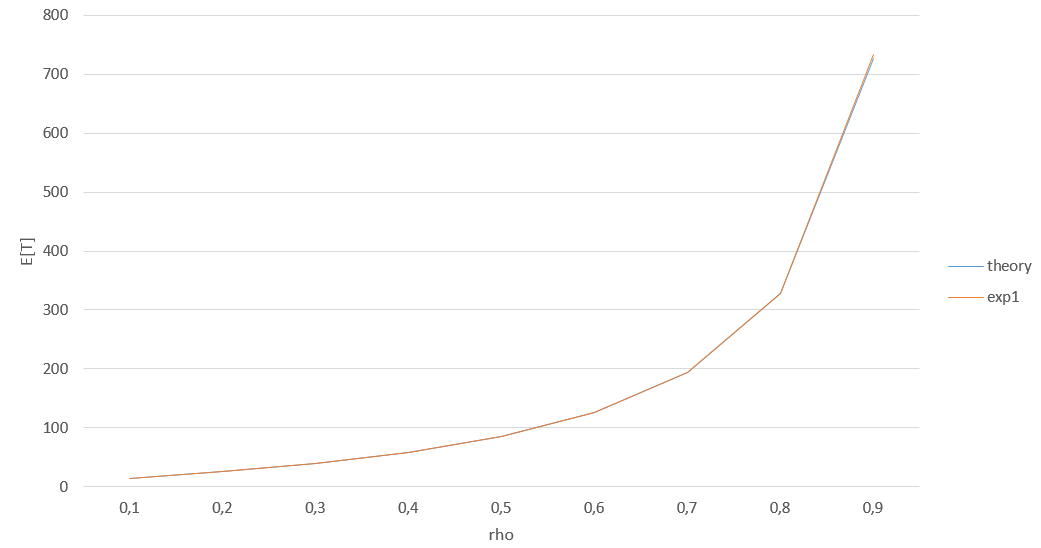
\includegraphics[scale=.5]{FCFS.PNG}
\end{center}
\caption{M/G/1/FCFS}
\end{figure}

\subsubsection{Conclusion}
The simulation perfectly fits the theoretical expectations : the biggest error (for highest $\rho$) is here strictly smaller than 1\%.
%---------------------------------------------------------------------------
\newpage
\subsection*{Question 2}
The only difference is in the implementation of the method \texttt{getFirst()} : it splits the items between those which need small time to be served and the others which need long time to be served. The order of arrival is kept in these two sub-lists. The queue will first look for a small "jobs", if this list is empty, it looks for a big one.

\subsubsection*{Theoretical predictions}

Let first derive the mean time of waiting (queuing and service) of small jobs : 
\begin{align*}
\mathbb{E}[T_{Q}^{s}] &= \rho \mathbb{E}[S_{E}] + \mathbb{E}[N_{Q}^{s}] \mathbb{E}[S_{s}] \\
&= \rho \mathbb{E}[S_{E}] + \mathbb{E}[T_{Q}^{s}] (0.98 \lambda \mathbb{E}[S_{s}])
\end{align*}

Thus :

\begin{equation}
\mathbb{E}[T_{Q}^{s}](1-0.98 \lambda \mathbb{E}[S_{s}]) = \rho \mathbb{E}[S_{E}]
\label{short}
\end{equation}

Let now derive the mean time of waiting (queuing and service) of long jobs : 

\[\mathbb{E}[T_{Q}^{l}] = \rho \mathbb{E}[S_{E}] + \mathbb{E}[N_{Q}] \mathbb{E}[S]+\mathbb{E}[T_{Q}^{l}] (0.98 \lambda \mathbb{E}[S_{s}])\]

So we get :

\begin{equation}
\mathbb{E}[T_{Q}^{l}](1-0.98 \lambda \mathbb{E}[S_{s}]) = \rho \mathbb{E}[S_{E}]+\rho \mathbb{E}[T_{Q}]
\label{long}
\end{equation}
\medbreak
In the equation $\eqref{result}\leftarrow 0.98 \times \eqref{short}+0.02 \times \eqref{long}$ :

\begin{equation}
\mathbb{E}[T_{Q}](1-0.98 \lambda \mathbb{E}[S_{s}]) = \rho \mathbb{E}[S_{E}]+0.02\rho \mathbb{E}[T_{Q}]
\label{result}
\end{equation}
\medbreak
Let set $\rho^{\star} = (0.98 \frac{\mathbb{E}[S_{s}]}{\mathbb{E}[S]}+0.02) \rho$. 
\par
Thus, \eqref{result} is equivalent to :


\[\mathbb{E}[T_{Q}]=\frac{\rho}{1-\rho^{\star}}\frac{\mathbb{E}[S^{2}]}{2 \mathbb{E}[S]}\]

In conclusion,

\[\mathbb{E}[T]^{M/G/1/SJF}=\frac{\rho}{1-\rho^{\star}}\frac{\mathbb{E}[S^{2}]}{2 \mathbb{E}[S]}+\mathbb{E}[S]\]

where $\mathbb{E}[S] = 5s$ and $\mathbb{E}[S^{2}] = 809 s^{2}$.

\subsubsection*{Experimental results}

\begin{center}
\begin{tabular}{|c|c|c|}

\hline
\ $\rho$ & \textbf{Theory} & \textbf{Experiment}  \\
\hline
0.1 & 13.269 & 13.267  \\
\hline
0.2 & 21.911 & 21.926  \\
\hline
0.3 & 30.952 & 30.999  \\
\hline
0.4 & 40.420 & 40.578  \\
\hline
0.5 & 50.348 &  50.775 \\
\hline
0.6 & 60.768 & 61.631  \\
\hline
0.7 & 71.718 & 73.662  \\
\hline
0.8 & 83.240 & 87.879  \\
\hline
0.9 & 95.380 & 109.210  \\
\hline

\end{tabular}
\end{center}


\begin{figure}[ht]
\begin{center}
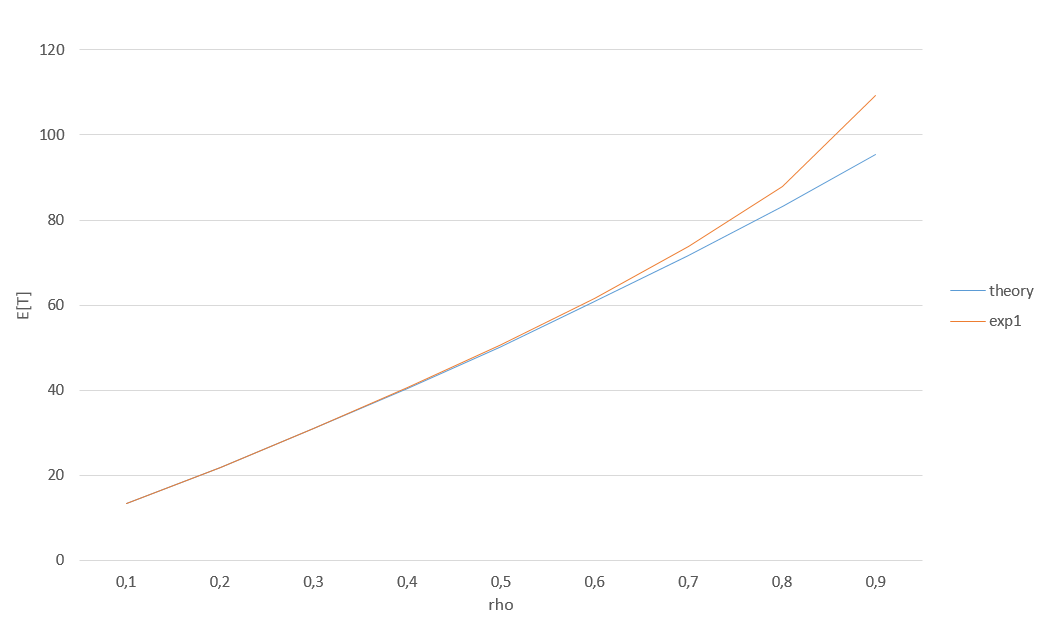
\includegraphics[scale=.5]{SJF.PNG}
\end{center}
\caption{M/G/1/SJF}
\end{figure}

\subsubsection{Conclusion}
The experiment fits here a bit less to the theory than it fitted in the first case: as soon as $\rho$ is greater than 0.6 / 0.7, the error rate exploded from around to 1\% to 14\% (for highest $\rho$). Actually, I don't really understand why there is such an explosion : I ran twice the simulation and got "exactly" the same result. The problem is not a problem of convergence. Thus it could a problem laying either in the way I coded the program or in the way I built my theoretical predictions. First question validated all the code for a M/G/1/FCFS queue : so, if it is really a coding mistake, the error can only be in the scheduling method \texttt{getFirstItem()} (but I can't understand where). Or maybe it's a theoretical mistake. Nonetheless, why the theory would be validated for low utilization but not high one ?

\begin{figure}[ht]
\begin{center}
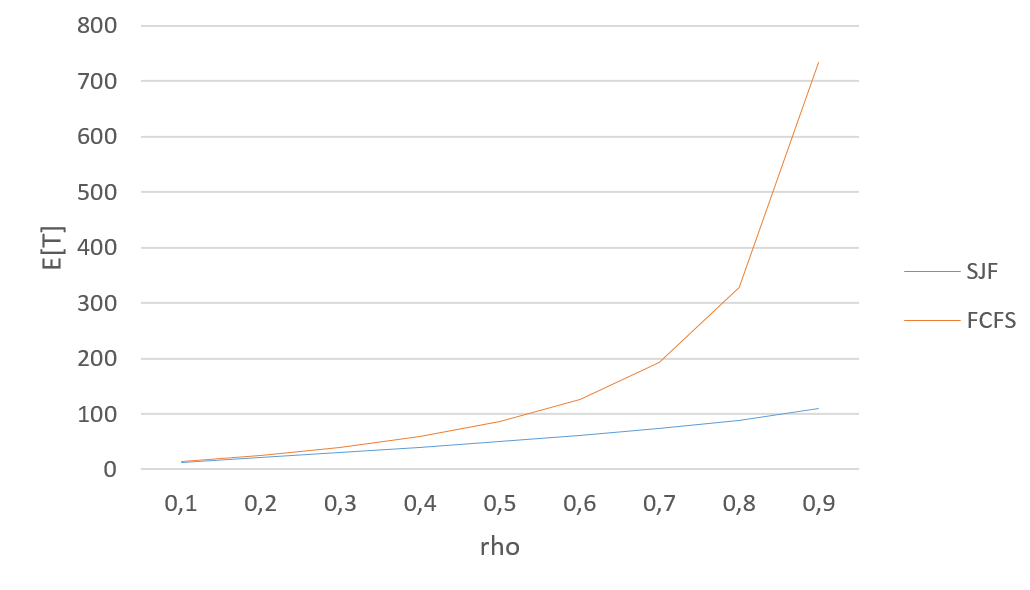
\includegraphics[scale=.5]{Comp.PNG}
\end{center}
\caption{Comparison between M/G/1/FCFS and M/G/1/SJF}
\end{figure}

\medbreak
However, we can notice that the SJF scheduling is far more effective than the FCFS one.

\end{document}